% Options for packages loaded elsewhere
\PassOptionsToPackage{unicode}{hyperref}
\PassOptionsToPackage{hyphens}{url}
%
\documentclass[
  12pt,a4paper,lualatex,ja=standard]{bxjsarticle}
\usepackage{lmodern}
\usepackage{amsmath}
\usepackage{ifxetex,ifluatex}
\ifnum 0\ifxetex 1\fi\ifluatex 1\fi=0 % if pdftex
  \usepackage[T1]{fontenc}
  \usepackage[utf8]{inputenc}
  \usepackage{textcomp} % provide euro and other symbols
  \usepackage{amssymb}
\else % if luatex or xetex
  \usepackage{unicode-math}
  \defaultfontfeatures{Scale=MatchLowercase}
  \defaultfontfeatures[\rmfamily]{Ligatures=TeX,Scale=1}
\fi
% Use upquote if available, for straight quotes in verbatim environments
\IfFileExists{upquote.sty}{\usepackage{upquote}}{}
\IfFileExists{microtype.sty}{% use microtype if available
  \usepackage[]{microtype}
  \UseMicrotypeSet[protrusion]{basicmath} % disable protrusion for tt fonts
}{}
\makeatletter
\@ifundefined{KOMAClassName}{% if non-KOMA class
  \IfFileExists{parskip.sty}{%
    \usepackage{parskip}
  }{% else
    \setlength{\parindent}{0pt}
    \setlength{\parskip}{6pt plus 2pt minus 1pt}}
}{% if KOMA class
  \KOMAoptions{parskip=half}}
\makeatother
\usepackage{xcolor}
\IfFileExists{xurl.sty}{\usepackage{xurl}}{} % add URL line breaks if available
\IfFileExists{bookmark.sty}{\usepackage{bookmark}}{\usepackage{hyperref}}
\hypersetup{
  hidelinks,
  pdfcreator={LaTeX via pandoc}}
\urlstyle{same} % disable monospaced font for URLs
\usepackage{graphicx}
\makeatletter
\def\maxwidth{\ifdim\Gin@nat@width>\linewidth\linewidth\else\Gin@nat@width\fi}
\def\maxheight{\ifdim\Gin@nat@height>\textheight\textheight\else\Gin@nat@height\fi}
\makeatother
% Scale images if necessary, so that they will not overflow the page
% margins by default, and it is still possible to overwrite the defaults
% using explicit options in \includegraphics[width, height, ...]{}
\setkeys{Gin}{width=\maxwidth,height=\maxheight,keepaspectratio}
% Set default figure placement to htbp
\makeatletter
\def\fps@figure{htbp}
\makeatother
\setlength{\emergencystretch}{3em} % prevent overfull lines
\providecommand{\tightlist}{%
  \setlength{\itemsep}{0pt}\setlength{\parskip}{0pt}}
\setcounter{secnumdepth}{5}
\usepackage{indentfirst}
\parindent = 1em
\usepackage{dcolumn}
\newcolumntype{.}{D{.}{.}{-1}}
\usepackage{caption}
\captionsetup[table]{name=表}
\captionsetup[figure]{name=図}
\usepackage{hyperref}
\pagestyle{empty}
\usepackage{multicol}
\usepackage{ascmac}
\setpagelayout*{top=10truemm,bottom=30truemm,left=10truemm,right=10truemm}
\usepackage{tikz}
\usetikzlibrary{arrows.meta,decorations,decorations.pathreplacing,arrows,calc}
\usepackage{tabstackengine}
\usepackage{xcolor}
\usepackage{rotating}
\usepackage{txfonts}
\usepackage{fancybox}
\usepackage{dashbox}
\usepackage{tcolorbox}
\tcbuselibrary{theorems,skins}
\usepackage{siunitx}
\usepackage{framed}
\usepackage{enumerate}
\usepackage{lastpage}
\usepackage{pgfplots}
\pgfplotsset{compat=1.15}
\usepackage{mathrsfs}
\ifluatex
  \usepackage{selnolig}  % disable illegal ligatures
\fi

\author{}
\date{\vspace{-2.5em}}

\begin{document}

\renewcommand{\thefootnote}{}
\newcounter{kaunta}
\renewcommand{\thekaunta}{\arabic{kaunta}}
\newcommand{\kaunta}{\refstepcounter{kaunta}%
\thekaunta}
\def\question{\noindent\fbox{\large\makebox[1em]{\text{\kaunta}}} \hspace{1pt}}
\newcounter{skaunta}
\renewcommand{\theskaunta}{\arabic{skaunta}}
\newcommand{\skaunta}{\refstepcounter{skaunta}%
\theskaunta}
\def\squestion{(\text{\skaunta})\hspace{2.5pt}}
\newcommand{\maru}[1]{\raise0.2ex\hbox{\textcircled{\scriptsize{#1}}}}
\newcommand{\jsim}{\mathrel{\text{∽}}}
\newcommand{\jpara}{/\!/}
\newcounter{kurankaunta}
\renewcommand{\thekurankaunta}{\arabic{kurankaunta}}
\newcommand{\kurankaunta}{\refstepcounter{kurankaunta}%
\thekurankaunta}

\newcounter{kcounter}
\setcounter{kcounter}{0}
\newcommand{\kana}{\refstepcounter{kcounter}\ifthenelse{\value{kcounter}=1}{ア}{\ifthenelse{\value{kcounter}=2}{イ}{\ifthenelse{\value{kcounter}=3}{ウ}{\ifthenelse{\value{kcounter}=4}{エ}{\ifthenelse{\value{kcounter}=5}{オ} {\ifthenelse{\value{kcounter}=6}{カ}{\ifthenelse{\value{kcounter}=7}{キ}{\ifthenelse{\value{kcounter}=8}{ク}{\ifthenelse{\value{kcounter}=9}{ケ}{\ifthenelse{\value{kcounter}=10}{コ}{\ifthenelse{\value{kcounter}=11}{サ}{\ifthenelse{\value{kcounter}=12}{シ}{\ifthenelse{\value{kcounter}=13}{ス}{\ifthenelse{\value{kcounter}=14}{セ}{\ifthenelse{\value{kcounter}=15}{ソ}{\ifthenelse{\value{kcounter}=16}{タ}{\ifthenelse{\value{kcounter}=17}{チ}{\ifthenelse{\value{kcounter}=18}{ツ}{\ifthenelse{\value{kcounter}=19}{テ}{\ifthenelse{\value{kcounter}=20}{ト}{\ifthenelse{\value{kcounter}=21}{ナ}{\ifthenelse{\value{kcounter}=22}{ニ}{\ifthenelse{\value{kcounter}=23}{ヌ}{\ifthenelse{\value{kcounter}=24}{ネ}{\ifthenelse{\value{kcounter}=25}{ノ}{\ifthenelse{\value{kcounter}=26}{ハ}{\ifthenelse{\value{kcounter}=27}{ヒ}{\ifthenelse{\value{kcounter}=28}{フ}{\ifthenelse{\value{kcounter}=29}{ヘ}{\ifthenelse{\value{kcounter}=30}{ホ}{\ifthenelse{\value{kcounter}=31}{マ}{\ifthenelse{\value{kcounter}=32}{ミ}{\ifthenelse{\value{kcounter}=33}{ム}{\ifthenelse{\value{kcounter}=34}{メ}{\ifthenelse{\value{kcounter}=35}{モ}{\ifthenelse{\value{kcounter}=36}{ヤ}{\ifthenelse{\value{kcounter}=37}{ユ}{\ifthenelse{\value{kcounter}=38}{ヨ}{\ifthenelse{\value{kcounter}=39}{ラ}{\ifthenelse{\value{kcounter}=40}{リ}{\ifthenelse{\value{kcounter}=41}{ル}{\ifthenelse{\value{kcounter}=42}{レ}{\ifthenelse{\value{kcounter}=43}{ロ}{\ifthenelse{\value{kcounter}=44}{ワ}{・}}}}}}}}}}}}}}}}}}}}}}}}}}}}}}}}}}}}}}}}}}}}}

\newcommand{\kuran}[1]{\framebox[1.5cm][c]{\maru{\kana}}}
\newcommand{\sukuran}[1]{\framebox[1.5cm][c]{\maru{\kurankaunta}}}

\newcommand{\degre}{\ensuremath{^\circ}}

\newcommand{\myarc}[1]{
   \tikz [baseline = (N.base), every node/.style={}] {
      \node [inner sep = 0pt] (N) {$\mathrm{#1}$};
      \draw [line width = 0.4pt] plot [smooth, tension=1.3] coordinates {
         ($(N.north west) + (0.1ex,0)$)
         ($(N.north)      + (0,0.5ex)$)
         ($(N.north east) + (0,0)$)
      };
   }
}

\makeatletter
\newenvironment{figurehere}{\def\@captype{figure}}{}
\makeatother

\newcommand{\haiten}[1]{%
\begin{flushright}%
\footnotesize{<#1>}%
\end{flushright}%
}

\newcommand{\goku}[1]{\fbox{\phantom{\text{#1}} \quad}}

\newgeometry{top=10truemm,bottom=10truemm,left=20truemm,right=20truemm}

\thispagestyle{empty}
\begin{center}
\phantom{empty}

\vspace{60truemm}

\hspace{4em} {\HUGE\gtfamily\bfseries 数\hspace{2em}学}\hspace{1em}{\large \gtfamily \bfseries ($\mathbf{2}$年)}\\

\vspace{15truemm}

%\hspace{2.5em}{\large \gtfamily \bfseries (この問題は定規とコンパスが必要です。)}

\vspace{64truemm}

{\large\gtfamily\bfseries 注\hspace{5em}意}

\end{center}

\centering
\begin{framed}
\begin{flushleft}
\begin{enumerate}[\Large \gtfamily 1]
  \item {\large 「開始」の合図があるまでは,開いてはいけません。}

  \item {\large 問題は\pageref{LastPage}ページまであります。}

  \item {\large 「開始」の合図があったら,まず,問題用紙・解答用紙に,組・番号と名前などを書きなさい。}

  \item {\large 答えは,すべて解答用紙に書きなさい。また、所定の欄に濃くはっきりと書きなさい。}

  \item {\large 「終了」の合図で,すぐ鉛筆をおき,解答用紙を裏返しにしなさい。}
\end{enumerate}
\end{flushleft}
\end{framed}

\vspace{14mm}

\begin{center}
{\large \underline{\hspace{30mm}組 \hspace{30mm}番 \hspace{15mm} 名前 \hspace{60mm}}}
\end{center}

\newpage

  \href{空白ページのための全角スペースあり。}{} \newpage

\pagestyle{plain}
\pagenumbering{arabic}

\begin{flushleft}

\noindent\fbox{\large\makebox[1em]{\text{\refstepcounter{kaunta}%
\arabic{kaunta}}}} \hspace{1pt}平行四辺形の定義をかけ。また、平行四辺形の性質を3つかけ。

%
\begin{flushright}%
\footnotesize{<知・技$2\times 4$点>}%
\end{flushright}%


\vfill

\noindent\fbox{\large\makebox[1em]{\text{\refstepcounter{kaunta}%
\arabic{kaunta}}}} \hspace{1pt}次の四角形は平行四辺形である。$x, \, y$の値を求めよ。

%
\begin{flushright}%
\footnotesize{<知・技$4\times 4$点>}%
\end{flushright}%


\begin{multicols}{2}
(\text{\refstepcounter{skaunta}%
\arabic{skaunta}})\hspace{2.5pt}

\begin{center}
\def\@captype{figure}
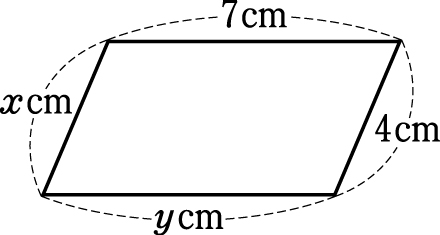
\includegraphics[height=30mm]{img/img1.jpg}

\end{center}

\columnbreak

(\text{\refstepcounter{skaunta}%
\arabic{skaunta}})\hspace{2.5pt}

\begin{center}
\def\@captype{figure}
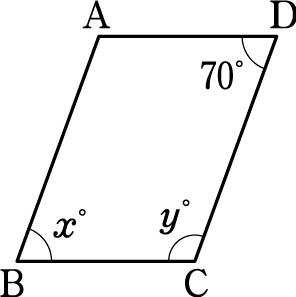
\includegraphics[height=30mm]{img/img2.jpg}

\end{center}

\end{multicols}

\vspace{5mm}

\begin{multicols}{2}
(\text{\refstepcounter{skaunta}%
\arabic{skaunta}})\hspace{2.5pt}

\begin{center}
\def\@captype{figure}
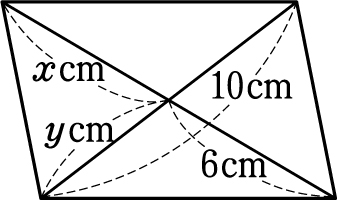
\includegraphics[height=30mm]{img/img3.jpg}

\end{center}

\columnbreak

(\text{\refstepcounter{skaunta}%
\arabic{skaunta}})\hspace{2.5pt}

\begin{center}
\def\@captype{figure}
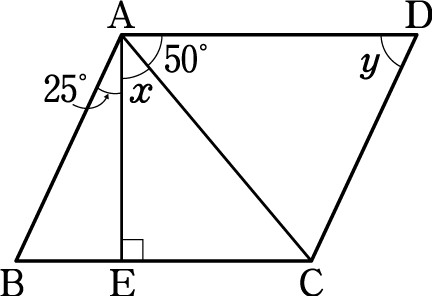
\includegraphics[height=30mm]{img/img4.jpg}

\end{center}

\end{multicols}

\setcounter{skaunta}{0}

\vspace{5mm}

\noindent\fbox{\large\makebox[1em]{\text{\refstepcounter{kaunta}%
\arabic{kaunta}}}} \hspace{1pt}次の空欄に当てはまる数字や式を答えなさい。

%
\begin{flushright}%
\footnotesize{<知・技$3 \times 3$点>}%
\end{flushright}%


(\text{\refstepcounter{skaunta}%
\arabic{skaunta}})\hspace{2.5pt}かならず起こることがらの確率は\fbox{\phantom{\text{1}} \quad}である。

(\text{\refstepcounter{skaunta}%
\arabic{skaunta}})\hspace{2.5pt}けっして起こらないことがらの確率は\fbox{\phantom{\text{0}} \quad}である。

(\text{\refstepcounter{skaunta}%
\arabic{skaunta}})\hspace{2.5pt}ことがらAの起こる確率を$p$とすると、

$$
\mbox{(Aの起こらない確率)} = \fbox{\phantom{\text{1ーp}} \quad}
$$
である。

\vfill

\setcounter{skaunta}{0}

\noindent\fbox{\large\makebox[1em]{\text{\refstepcounter{kaunta}%
\arabic{kaunta}}}} \hspace{1pt}1つのさいころを投げるとき、1の目が出る確率は$\frac{1}{6}$です。この確率の意味を正しく説明しているのは、次の$\raise 0.2ex\hbox{\textcircled{\scriptsize{ア}}} \sim \raise 0.2ex\hbox{\textcircled{\scriptsize{ウ}}}$のうち、どれですか。

%
\begin{flushright}%
\footnotesize{<知・技3点>}%
\end{flushright}%


\begin{itemize}
\item[\raise 0.2ex\hbox{\textcircled{\scriptsize{ア}}}] 6回投げるとき、そのうち、1回はかならず1の目が出る。

\item[\raise 0.2ex\hbox{\textcircled{\scriptsize{イ}}}] 6回投げるとき、そのうち1回しか1の目は出ない。

\item[\raise 0.2ex\hbox{\textcircled{\scriptsize{ウ}}}] 3000回投げるとき、500回ぐらい1の目が出る。
\end{itemize}

\vfill

\newpage

\noindent\fbox{\large\makebox[1em]{\text{\refstepcounter{kaunta}%
\arabic{kaunta}}}} \hspace{1pt}500円玉、100円玉、50円玉の3枚の硬貨を同時に投げます。次の問に答えなさい。

%
\begin{flushright}%
\footnotesize{<知・技$3\times 4$点>}%
\end{flushright}%


(\text{\refstepcounter{skaunta}%
\arabic{skaunta}})\hspace{2.5pt}表裏の出方は何通りありますか。

\vspace{10mm}

(\text{\refstepcounter{skaunta}%
\arabic{skaunta}})\hspace{2.5pt}1枚だけ表になる確率

\vspace{10mm}

(\text{\refstepcounter{skaunta}%
\arabic{skaunta}})\hspace{2.5pt}3枚とも裏となる確率

\vspace{10mm}

(\text{\refstepcounter{skaunta}%
\arabic{skaunta}})\hspace{2.5pt}少なくとも1枚は表となる確率

\vspace{10mm}

\vfill

\setcounter{skaunta}{0}

\noindent\fbox{\large\makebox[1em]{\text{\refstepcounter{kaunta}%
\arabic{kaunta}}}} \hspace{1pt}1から20までの数が1つずつ書かれた20枚のカードがあります。このカードを箱に入れて、カードを取り出します。次の問に答えなさい。

%
\begin{flushright}%
\footnotesize{<知・技$3\times 3$点>}%
\end{flushright}%


(\text{\refstepcounter{skaunta}%
\arabic{skaunta}})\hspace{2.5pt}1枚のカードを取り出すとき、取り出したカードが23である確率を求めなさい。

\vspace{10mm}

(\text{\refstepcounter{skaunta}%
\arabic{skaunta}})\hspace{2.5pt}1枚のカードを取り出すとき、取り出したカードが3の倍数である確率を求めなさい。

\vspace{10mm}

(\text{\refstepcounter{skaunta}%
\arabic{skaunta}})\hspace{2.5pt}2枚のカードを取り出すとき、取り出したカードの和が5になる確率を求めなさい。

\vspace{10mm}

\vfill

\setcounter{skaunta}{0}

\noindent\fbox{\large\makebox[1em]{\text{\refstepcounter{kaunta}%
\arabic{kaunta}}}} \hspace{1pt}次の確率を求めなさい。

%
\begin{flushright}%
\footnotesize{<知・技$3\times 2$点>}%
\end{flushright}%


(\text{\refstepcounter{skaunta}%
\arabic{skaunta}})\hspace{2.5pt}大小2つのさいころを投げるとき、目の和が7になる確率。

\vspace{10mm}

(\text{\refstepcounter{skaunta}%
\arabic{skaunta}})\hspace{2.5pt}赤玉4個、黄玉2個、青玉3個がはいっている箱から玉を1個取り出すとき、赤玉が出る確率。

\vspace{10mm}

\vfill
\newpage

\setcounter{skaunta}{0}

\noindent\fbox{\large\makebox[1em]{\text{\refstepcounter{kaunta}%
\arabic{kaunta}}}} \hspace{1pt}A, B, C, Dの4つのグループが10点満点のゲームを行いました。

%
\begin{flushright}%
\footnotesize{<知・技(1)8点、(2)3点、(3)6点、(4)(5)3点>}%
\end{flushright}%


(\text{\refstepcounter{skaunta}%
\arabic{skaunta}})\hspace{2.5pt}Aグループの得点は下のようになりました。四分位数と四分位範囲をそれぞれ求めなさい。

$$
3\quad 4\quad 9\quad 3\quad 6\quad 5\quad 7 \qquad \mbox{(単位 点)}
$$

\vfill

(\text{\refstepcounter{skaunta}%
\arabic{skaunta}})\hspace{2.5pt}Bグループの四分位数と最大値、最小値は下の表のようになりました。これらの値をもとに、下の図の箱ひげ図をかき入れなさい。(単位 点)

\begin{center}
\begin{tabular}{|c|c|c|c|c|}
\hline
最小値 & 第1四分位数 & %
\begin{tabular}{c}%
中央値\\(第2四分位数)%
\end{tabular}%
& 第3四分位数 & 最大値 \\
\hline
1 & 3 & 4 & 5 & 7 \\
\hline
\end{tabular}

\def\@captype{figure}
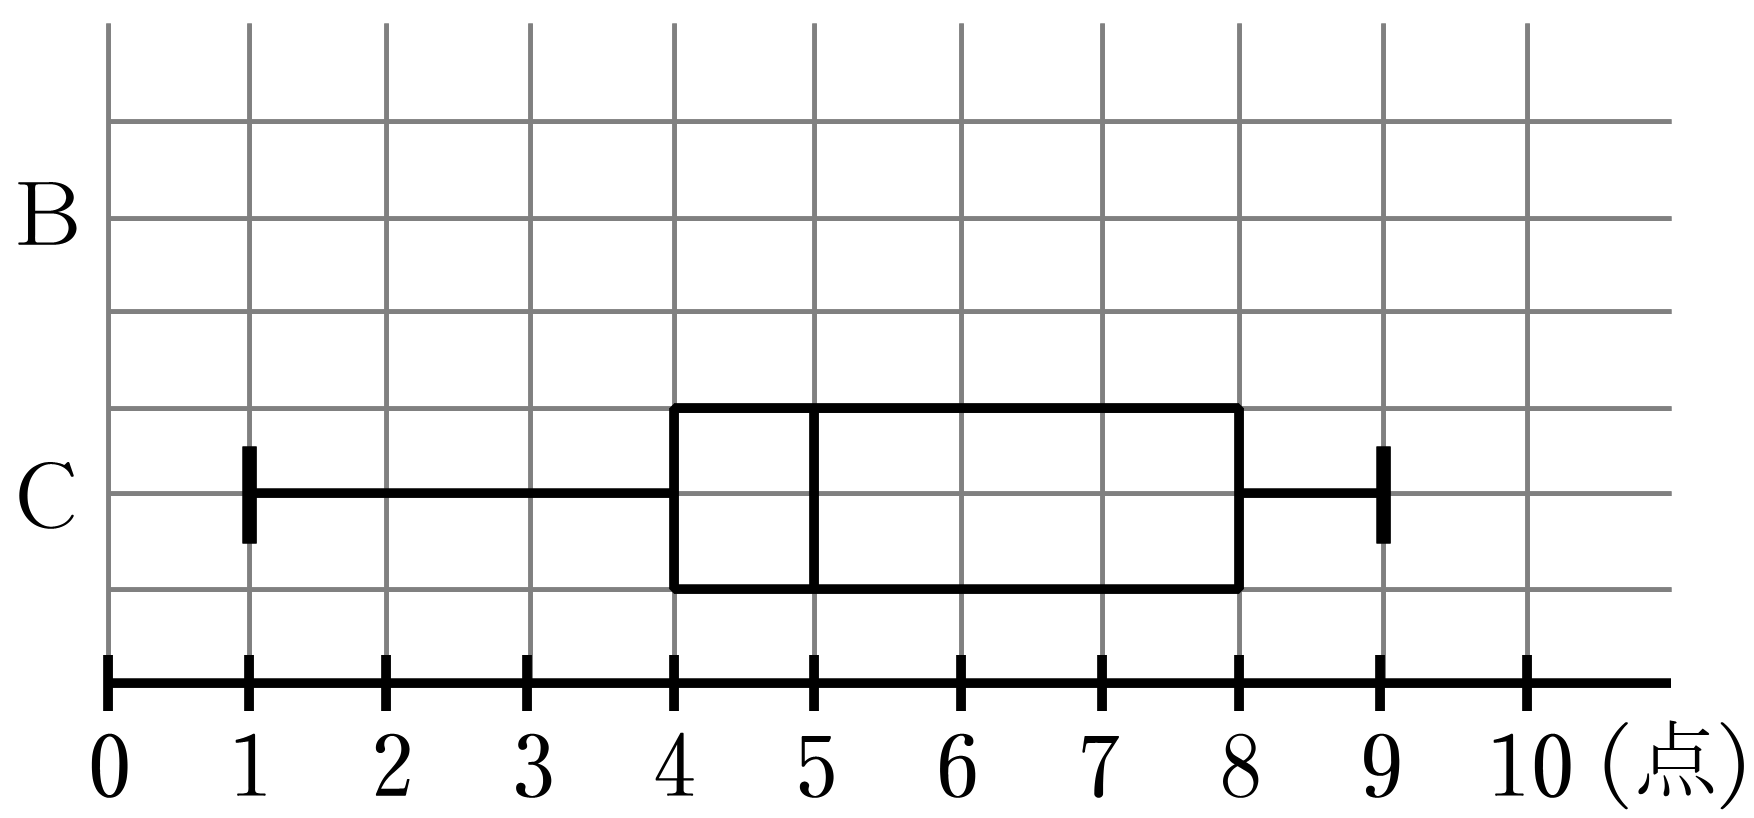
\includegraphics{img/image1.png}


\end{center}

\vspace{5mm}

(\text{\refstepcounter{skaunta}%
\arabic{skaunta}})\hspace{2.5pt}Cグループの箱ひげ図は、上の図のようになりました。箱ひげ図から中央値(第2四分位数)、四分位範囲、範囲を読み取りなさい。

\vfill

(\text{\refstepcounter{skaunta}%
\arabic{skaunta}})\hspace{2.5pt}四分位範囲や箱ひげ図からA, B, Cの3つのグループのうち、中央値のまわりの散らばりの程度が大きいのは、どのグループであるといえますか。

\vfill

\begin{multicols}{3}
(\text{\refstepcounter{skaunta}%
\arabic{skaunta}})\hspace{2.5pt}右の図は、Dグループの得点をヒストグラムに表したものです。これに対応する箱ひげ図を、ア$\sim$ウの中から選び、記号で答えなさい。

\columnbreak

\def\@captype{figure}
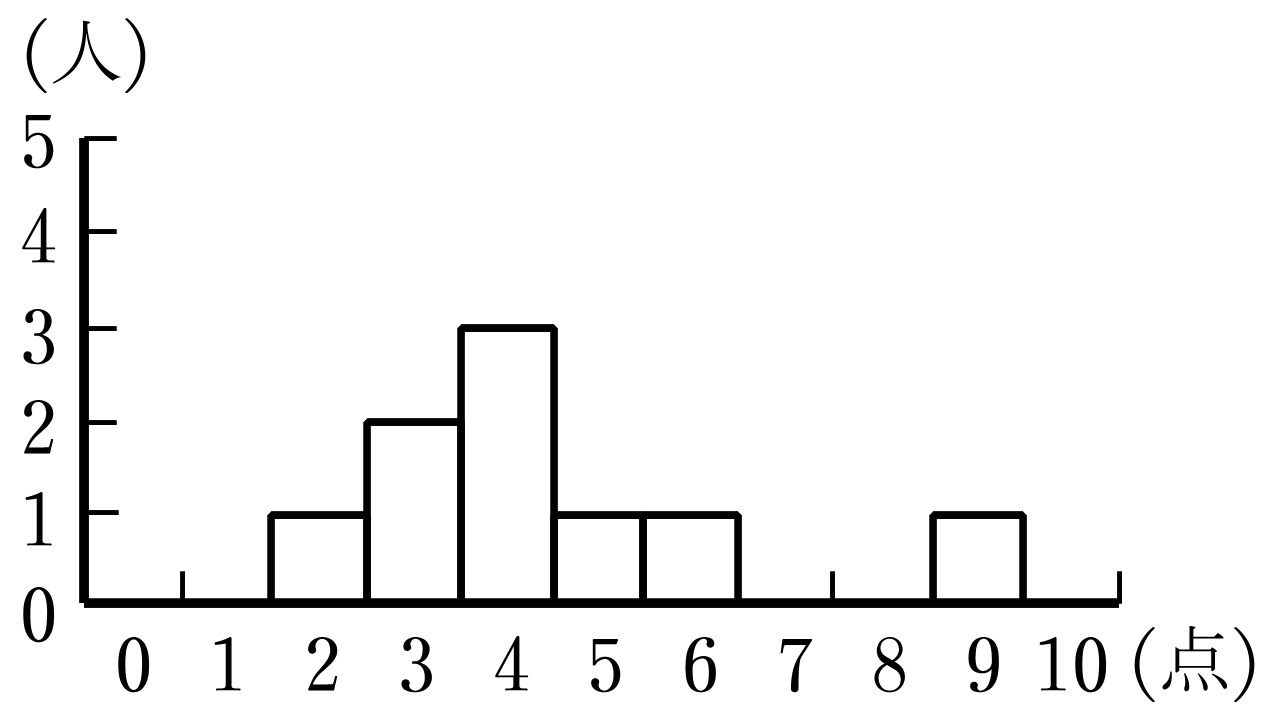
\includegraphics{img/image3.png}


\columnbreak

\def\@captype{figure}

\includegraphics{img/image2.png}


\end{multicols}

\vfill

\newpage

\setcounter{skaunta}{0}

\noindent\fbox{\large\makebox[1em]{\text{\refstepcounter{kaunta}%
\arabic{kaunta}}}} \hspace{1pt}下の箱ひげ図は、バスケットボール部のA, B, Cの3人が、最近の12試合で成功したシュートの本数を表したものです。この箱ひげ図について、次の問に答えなさい。

%
\begin{flushright}%
\footnotesize{<知・技(1)2点、思・判・表(2)4点>}%
\end{flushright}%


\begin{figure}
\centering

\includegraphics{img/image4.png}
\end{figure}

(\text{\refstepcounter{skaunta}%
\arabic{skaunta}})\hspace{2.5pt}次のことがらのうち、箱ひげ図から読み取れることとして、正しいものを1つ選び、記号で答えなさい。

\begin{itemize}
\item[\refstepcounter{kcounter}\ifthenelse{\value{kcounter}=1}{ア}{\ifthenelse{\value{kcounter}=2}{イ}{\ifthenelse{\value{kcounter}=3}{ウ}{\ifthenelse{\value{kcounter}=4}{エ}{\ifthenelse{\value{kcounter}=5}{オ} {\ifthenelse{\value{kcounter}=6}{カ}{\ifthenelse{\value{kcounter}=7}{キ}{\ifthenelse{\value{kcounter}=8}{ク}{\ifthenelse{\value{kcounter}=9}{ケ}{\ifthenelse{\value{kcounter}=10}{コ}{\ifthenelse{\value{kcounter}=11}{サ}{\ifthenelse{\value{kcounter}=12}{シ}{\ifthenelse{\value{kcounter}=13}{ス}{\ifthenelse{\value{kcounter}=14}{セ}{\ifthenelse{\value{kcounter}=15}{ソ}{\ifthenelse{\value{kcounter}=16}{タ}{\ifthenelse{\value{kcounter}=17}{チ}{\ifthenelse{\value{kcounter}=18}{ツ}{\ifthenelse{\value{kcounter}=19}{テ}{\ifthenelse{\value{kcounter}=20}{ト}{\ifthenelse{\value{kcounter}=21}{ナ}{\ifthenelse{\value{kcounter}=22}{ニ}{\ifthenelse{\value{kcounter}=23}{ヌ}{\ifthenelse{\value{kcounter}=24}{ネ}{\ifthenelse{\value{kcounter}=25}{ノ}{\ifthenelse{\value{kcounter}=26}{ハ}{\ifthenelse{\value{kcounter}=27}{ヒ}{\ifthenelse{\value{kcounter}=28}{フ}{\ifthenelse{\value{kcounter}=29}{ヘ}{\ifthenelse{\value{kcounter}=30}{ホ}{\ifthenelse{\value{kcounter}=31}{マ}{\ifthenelse{\value{kcounter}=32}{ミ}{\ifthenelse{\value{kcounter}=33}{ム}{\ifthenelse{\value{kcounter}=34}{メ}{\ifthenelse{\value{kcounter}=35}{モ}{\ifthenelse{\value{kcounter}=36}{ヤ}{\ifthenelse{\value{kcounter}=37}{ユ}{\ifthenelse{\value{kcounter}=38}{ヨ}{\ifthenelse{\value{kcounter}=39}{ラ}{\ifthenelse{\value{kcounter}=40}{リ}{\ifthenelse{\value{kcounter}=41}{ル}{\ifthenelse{\value{kcounter}=42}{レ}{\ifthenelse{\value{kcounter}=43}{ロ}{\ifthenelse{\value{kcounter}=44}{ワ}{・}}}}}}}}}}}}}}}}}}}}}}}}}}}}}}}}}}}}}}}}}}}}] 3人とも、9本成功した試合が、少なくとも1試合ある。
\item[\refstepcounter{kcounter}\ifthenelse{\value{kcounter}=1}{ア}{\ifthenelse{\value{kcounter}=2}{イ}{\ifthenelse{\value{kcounter}=3}{ウ}{\ifthenelse{\value{kcounter}=4}{エ}{\ifthenelse{\value{kcounter}=5}{オ} {\ifthenelse{\value{kcounter}=6}{カ}{\ifthenelse{\value{kcounter}=7}{キ}{\ifthenelse{\value{kcounter}=8}{ク}{\ifthenelse{\value{kcounter}=9}{ケ}{\ifthenelse{\value{kcounter}=10}{コ}{\ifthenelse{\value{kcounter}=11}{サ}{\ifthenelse{\value{kcounter}=12}{シ}{\ifthenelse{\value{kcounter}=13}{ス}{\ifthenelse{\value{kcounter}=14}{セ}{\ifthenelse{\value{kcounter}=15}{ソ}{\ifthenelse{\value{kcounter}=16}{タ}{\ifthenelse{\value{kcounter}=17}{チ}{\ifthenelse{\value{kcounter}=18}{ツ}{\ifthenelse{\value{kcounter}=19}{テ}{\ifthenelse{\value{kcounter}=20}{ト}{\ifthenelse{\value{kcounter}=21}{ナ}{\ifthenelse{\value{kcounter}=22}{ニ}{\ifthenelse{\value{kcounter}=23}{ヌ}{\ifthenelse{\value{kcounter}=24}{ネ}{\ifthenelse{\value{kcounter}=25}{ノ}{\ifthenelse{\value{kcounter}=26}{ハ}{\ifthenelse{\value{kcounter}=27}{ヒ}{\ifthenelse{\value{kcounter}=28}{フ}{\ifthenelse{\value{kcounter}=29}{ヘ}{\ifthenelse{\value{kcounter}=30}{ホ}{\ifthenelse{\value{kcounter}=31}{マ}{\ifthenelse{\value{kcounter}=32}{ミ}{\ifthenelse{\value{kcounter}=33}{ム}{\ifthenelse{\value{kcounter}=34}{メ}{\ifthenelse{\value{kcounter}=35}{モ}{\ifthenelse{\value{kcounter}=36}{ヤ}{\ifthenelse{\value{kcounter}=37}{ユ}{\ifthenelse{\value{kcounter}=38}{ヨ}{\ifthenelse{\value{kcounter}=39}{ラ}{\ifthenelse{\value{kcounter}=40}{リ}{\ifthenelse{\value{kcounter}=41}{ル}{\ifthenelse{\value{kcounter}=42}{レ}{\ifthenelse{\value{kcounter}=43}{ロ}{\ifthenelse{\value{kcounter}=44}{ワ}{・}}}}}}}}}}}}}}}}}}}}}}}}}}}}}}}}}}}}}}}}}}}}] 成功した本数が7本以下だった試合が最も少ないのはAさんである。
\item[\refstepcounter{kcounter}\ifthenelse{\value{kcounter}=1}{ア}{\ifthenelse{\value{kcounter}=2}{イ}{\ifthenelse{\value{kcounter}=3}{ウ}{\ifthenelse{\value{kcounter}=4}{エ}{\ifthenelse{\value{kcounter}=5}{オ} {\ifthenelse{\value{kcounter}=6}{カ}{\ifthenelse{\value{kcounter}=7}{キ}{\ifthenelse{\value{kcounter}=8}{ク}{\ifthenelse{\value{kcounter}=9}{ケ}{\ifthenelse{\value{kcounter}=10}{コ}{\ifthenelse{\value{kcounter}=11}{サ}{\ifthenelse{\value{kcounter}=12}{シ}{\ifthenelse{\value{kcounter}=13}{ス}{\ifthenelse{\value{kcounter}=14}{セ}{\ifthenelse{\value{kcounter}=15}{ソ}{\ifthenelse{\value{kcounter}=16}{タ}{\ifthenelse{\value{kcounter}=17}{チ}{\ifthenelse{\value{kcounter}=18}{ツ}{\ifthenelse{\value{kcounter}=19}{テ}{\ifthenelse{\value{kcounter}=20}{ト}{\ifthenelse{\value{kcounter}=21}{ナ}{\ifthenelse{\value{kcounter}=22}{ニ}{\ifthenelse{\value{kcounter}=23}{ヌ}{\ifthenelse{\value{kcounter}=24}{ネ}{\ifthenelse{\value{kcounter}=25}{ノ}{\ifthenelse{\value{kcounter}=26}{ハ}{\ifthenelse{\value{kcounter}=27}{ヒ}{\ifthenelse{\value{kcounter}=28}{フ}{\ifthenelse{\value{kcounter}=29}{ヘ}{\ifthenelse{\value{kcounter}=30}{ホ}{\ifthenelse{\value{kcounter}=31}{マ}{\ifthenelse{\value{kcounter}=32}{ミ}{\ifthenelse{\value{kcounter}=33}{ム}{\ifthenelse{\value{kcounter}=34}{メ}{\ifthenelse{\value{kcounter}=35}{モ}{\ifthenelse{\value{kcounter}=36}{ヤ}{\ifthenelse{\value{kcounter}=37}{ユ}{\ifthenelse{\value{kcounter}=38}{ヨ}{\ifthenelse{\value{kcounter}=39}{ラ}{\ifthenelse{\value{kcounter}=40}{リ}{\ifthenelse{\value{kcounter}=41}{ル}{\ifthenelse{\value{kcounter}=42}{レ}{\ifthenelse{\value{kcounter}=43}{ロ}{\ifthenelse{\value{kcounter}=44}{ワ}{・}}}}}}}}}}}}}}}}}}}}}}}}}}}}}}}}}}}}}}}}}}}}] 範囲、四分位範囲のどちらも、Bさんが最も大きい。
\end{itemize}

\vspace{10mm}

(\text{\refstepcounter{skaunta}%
\arabic{skaunta}})\hspace{2.5pt}3人の成功したシュートの本数の平均値は同じになります。3人のうち、1人を次の試合で使うとしたら、あなたならA, B, Cのだれを選びますか。また、その選手を選んだ理由を、箱ひげ図の特徴を比較して説明しなさい。

\vfill

\begin{multicols}{2}
\noindent\fbox{\large\makebox[1em]{\text{\refstepcounter{kaunta}%
\arabic{kaunta}}}} \hspace{1pt}右の図のような平行四辺形ABCDで、$\angle{\mbox{BAD}}$の二等分線と辺BCとの交点をEとします。このとき、
$$
\mbox{EC} + \mbox{CD} = \mbox{AD}
$$
となることを証明しなさい。

%
\begin{flushright}%
\footnotesize{<思・判・表8点>}%
\end{flushright}%


\columnbreak

\begin{center}
\def\@captype{figure}
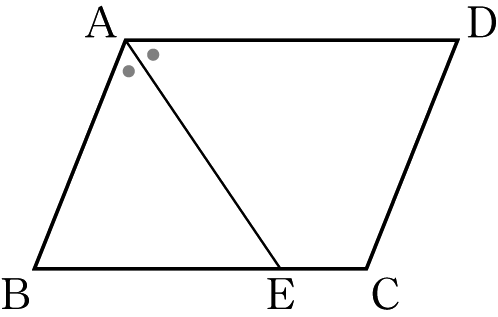
\includegraphics{img/image6.png}

\end{center}

\end{multicols}

\vfill

























\end{flushleft}

\end{document}
